\section{DeepSpeech}
Mozilla DeepSpeech is an end-to-end \gls{stt} model using tensorflow. It was first developed for translating English speech to English text \cite{Hannun2014DeepSS}. It is implemented using machine
translation techniques. \citet{Agarwal2019GermanES} have implemented a German \gls{stt} model using DeepSpeech. They provide all of their code and pre-trained models including ready-made scripts for
transfer-learning and fine-tuning \cite{Agarwal2019GermanES}. This avoids privacy issues of common web-services that require uploading potentially private data. Additionally, researchers are free to adjust and extend the model according to their requirements. DeepSpeech is a deep recurrent neural network (RNN) on character level. It can be trained using supervised learning.

\begin{figure}[h]
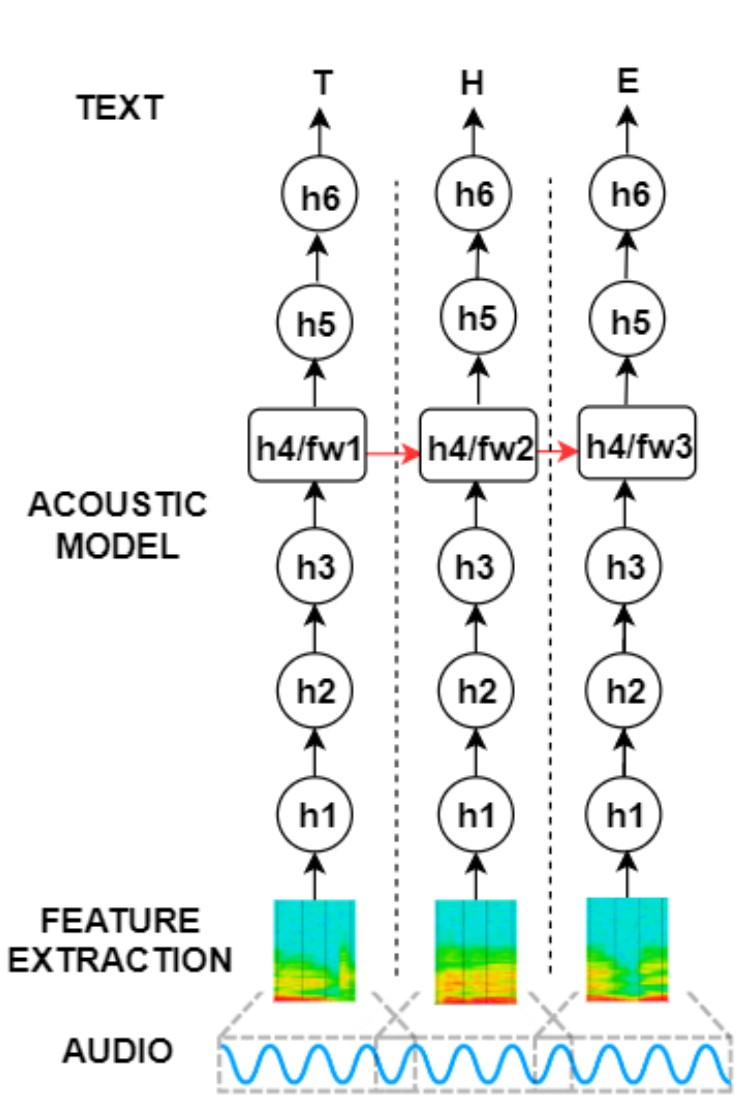
\includegraphics[scale=0.7]{deepspeech-de}
\caption{DeepSpeech architecture according to \citet{Agarwal2019GermanES}}
\label{architecture}
\end{figure}

The DeepSpeech architecture, as shown in figure \ref{architecture}, consists of 6 layers. The features extracted from the audio files are Frequency Cepstral Coefficients. Those essentially capture the frequency spectrum of an audio file in a condensed format. Those are fed to the first layer which is a fully connected, i.e. dense, layer like the next two. The fourth layer consists of unidirectional feed forward layer. The fifth layer is another dense layer which is followed by the output layer. A more in depth description can be found in \citet{Agarwal2019GermanES}. As becomes clear, the model has no additional phoneme-to-grapheme model but directly outputs the transcribed characters, respectively their probabilities. The Connectionist Temporal Classification (CTC) loss function is used to maximize the probability of the output characters. This loss is specifically designed for tasks where the prediction categories have unclear boundaries. In this case characters which can refer to phonemes that span over times frames of various length.
\\
The German DeepSpeech model integrates a language model that has to be built first. We trained it on two publicly available German datasets: One released by the University of Hamburg containing 8
million sentences \footnote{UHH Open source acoustic models - \url{https://www.inf.uni-hamburg.de/en/inst/ab/lt/resources/data/acoustic-models.html}} and the other the Europarl corpus containing another 2 million sentences
\footnote{Europarl - \url{https://www.statmt.org/europarl/}}.
